\documentclass[12pt]{article}
\usepackage[utf8]{inputenc}
\usepackage{graphicx}
\graphicspath{ {img/} }

\title{Grobkonzept \\ Automatisches finden von Fügepositionen}
\author{Özgür Gümüslü}
\date{März 2021}

\begin{document}
\maketitle
\tableofcontents
\newpage
\section{Aufgabenstellung}
In dieser Arbeit wird versucht im Rahmen des Kontextstudiums in der Digital Factory ein Verfahren zu
entwickeln welches es ermöglichen sollte ein Kugellager in ein Werkstück automatisch mittels eines
Kollaborativen Roboters der Firma Kuka (iiwa R700) einzufügen.

\section{Grober Überblick der Wissenschaft und Technik}
Kollaborative Roboter sind dafür ausgelegt ohne Schutzvorrichtungen mit Operatoren zusammen zu
Arbeiten. Diese können in verschiedenen Modis eingesetzt werden:

\begin{itemize}
\item Koexistierend \\
In dieser Form arbeiten Manipulator und Operator zeitlich und räumlich von einander getrennt.
 
\item Synchronisiert \\
Hier arbeiten sie im selben Raum, jedoch zeitlich voneinander getrennt.

\item Kooperativ \\
Hier abeiten sie räumlich und zeitlich zusammen, jedoch nicht am selben Bauteil.

\item Kollaborativ \\
Im Gegensatz wird hier am selben Bauteil gearbeitet.
\end{itemize}


Ein zentraler Aspekt ist dabei die Sicherheit. Der KUKA LBR iiwa 7 R800 verfügt über
Drehmomentensensoren die es erlaubt Kräfte in verschiedenen Achsen zu messen einerseits um sensitive
Arbeiten durchzuführen andererseits um Quetschungen und andere Gefärhdungen des Körperlichen Leibes
zu vermeiden.
\newpage
\subsection{Impedanzregelung}
Der Kontakt zwischen Roboter und Umgebung kann mittels der Hilfe der mechanischen Impedanz bzw. Feder-Dämpfer-Masse-System modeliert im Zeitbereich als
$f(t) = m \ddot{x(t)} + d \dot{x(t)} + c x(t)$ bzw.\\ im Bildbereich als $F(s) = (ms^2 + ds + c) X(s)$ werden.\\ Wobei folgendes für
\begin{itemize}
\item m ... Massenträgheitsmoment
\item d ... Dämpfung
\item c ... Steifigkeit
\end{itemize}
entspricht.[1]
\begin{center}
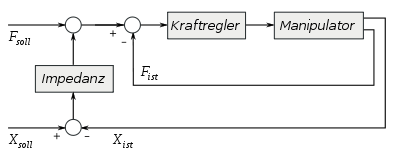
\includegraphics[scale=0.8]{img/Impedanzregler}\\
Postionsbasierte Impedanzregelung[2]
\end{center}
Mit Hilfe dieses Regelungskonzepts können Positionsänderungen mit Kräften und Drehmomenten in Beziehung gebracht werden.   


\subsection{Hybride Kraft-/Lageregelung}
Dieser besteht im wesentlichen aus zwei separaten Reglern. Hierfür wird der Raum in einen beschränkten und unbeschränkten Raum aufgeteilt. Im beschränkten Raum also in dem sich der Manipulator nicht frei bewegen kann, kommt der Kraftregler zum tragen. Im unbeschränkten Raum kommt der Lageregler zum Einsatz.
\begin{center}
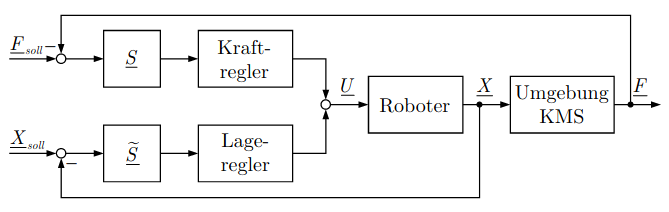
\includegraphics[scale=0.65]{img/Hybride_Kraft_Lageregelung}
Hybrider Kraft-/Lagereger [3]
\end{center}
Durch die Beschränkungen der Bewegungen und Kräfte lassen sich Selektionsmatrizen ableiten welche in der oberen Abbildung unter $\widetilde{\underline{S}}$ und $\underline{S}$ dargestellt werden.

\section{Komponenten}

\begin{center}
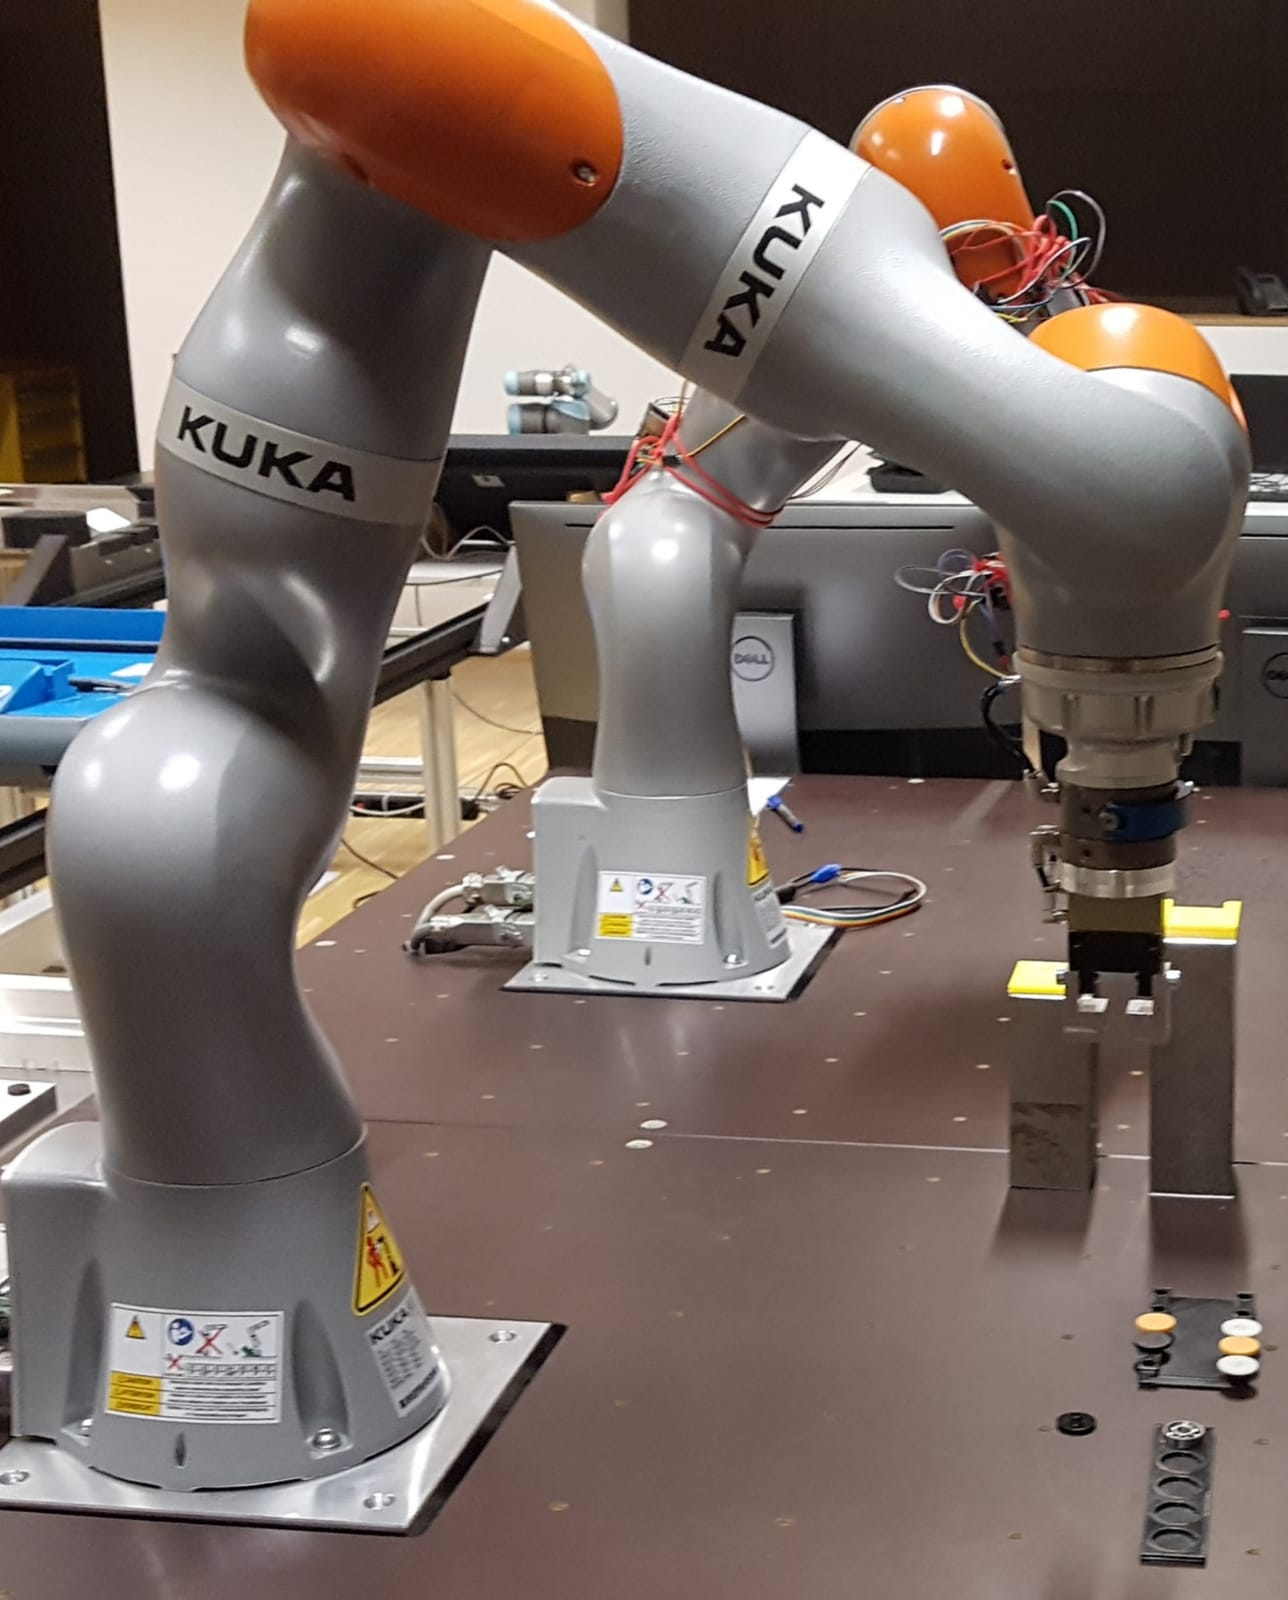
\includegraphics[width=0.5\textwidth]{img/Kuka}\\
Kollaborativer Roboter der Firma Kuka Modell LBR iiwa 7 R800\\
\end{center}


\begin{center}
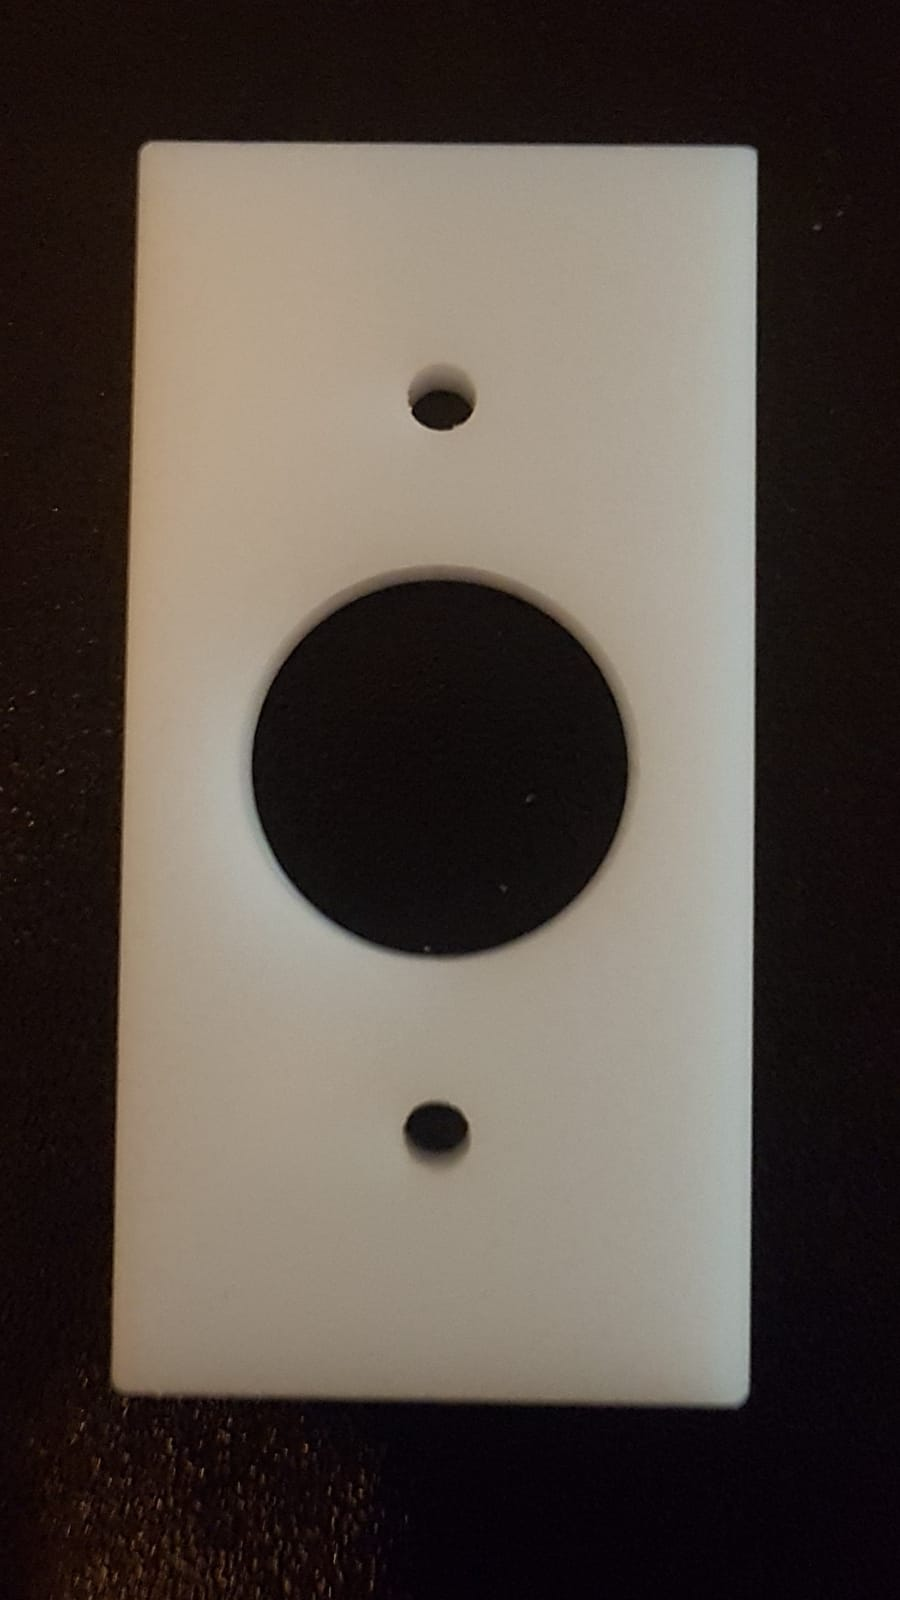
\includegraphics[width=0.2\textwidth]{img/werkstueck}\\
Werkstück 
\end{center}

\begin{center}
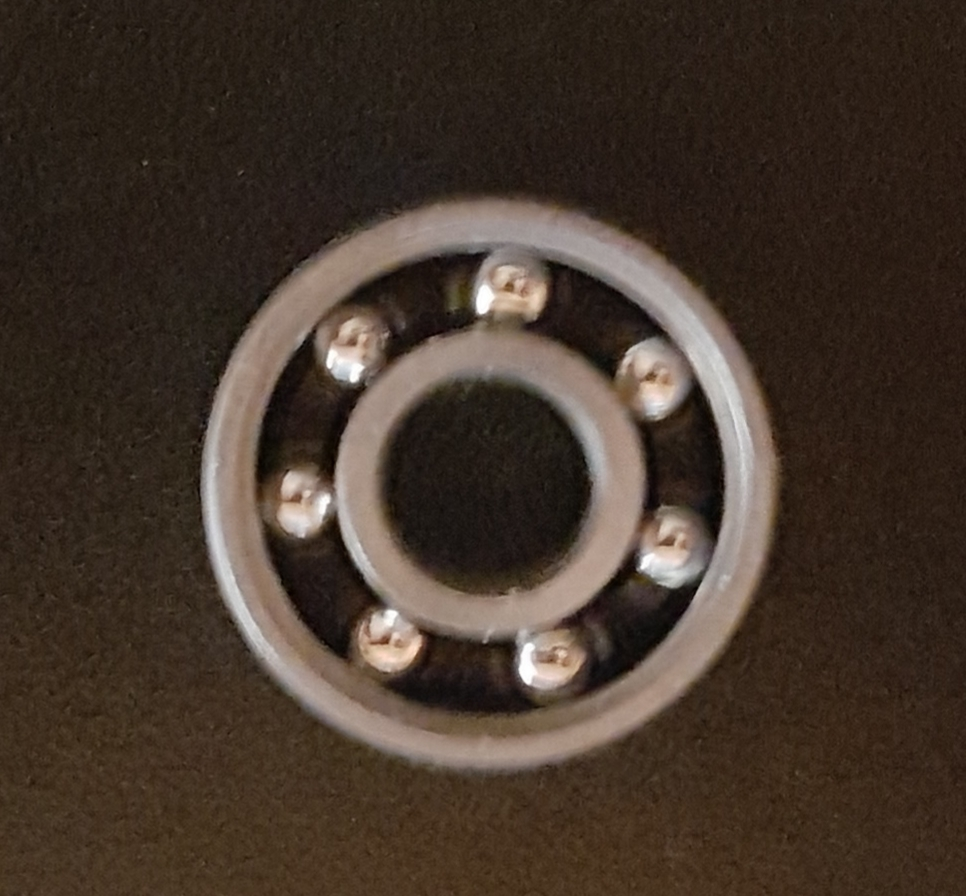
\includegraphics[width=0.3\textwidth]{img/Kugellager}\\
Fügeteil\\
\end{center}

\begin{center}
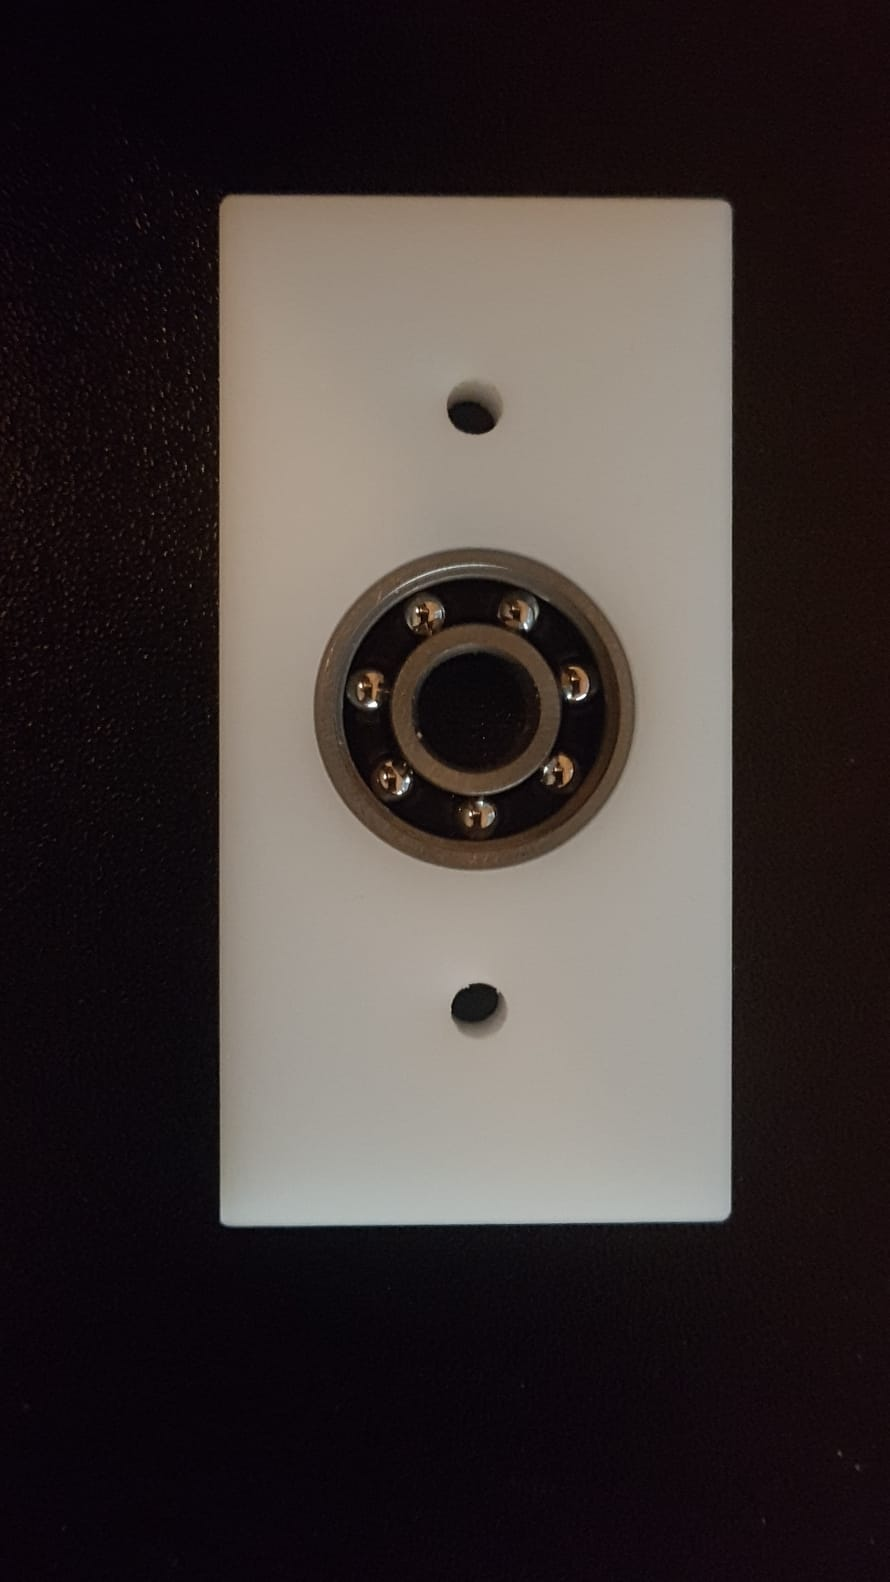
\includegraphics[width=0.3\textwidth]{img/montiertes_werkstueck}\\
Montiertes Werkstück
\end{center}

\newpage
\section{Konzept für die Umsetzung}

\begin{center}
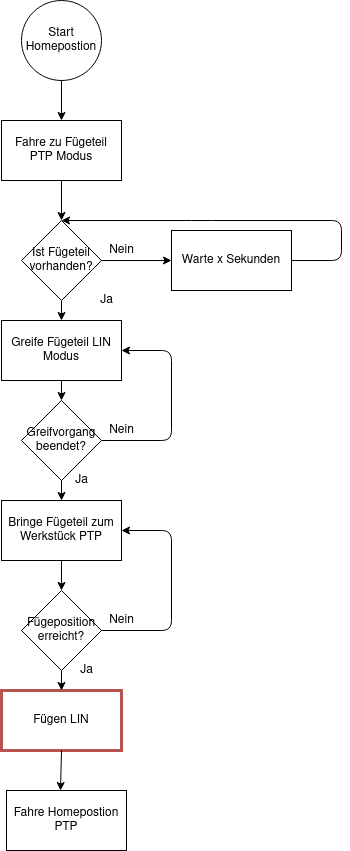
\includegraphics[scale=0.60]{img/Ablauf} \\
\end{center}

In der oberen Abbildung sollte ersichtlich sein wie dieser Prozess umgesetzt werden kann. Wie man sehen
kann wurde der "Fügen im Linear Verfahren Teil" rot markiert weil hier ein großes Augemerk in dieser Arbeit gelegt wird.
\subsection{Fügen}
Ist das Werkstück richtig positioniert stellt das Fügen kein Hinderniss dar. Doch was ist wenn das Werkstück
nicht optimal in der Fügeposition liegt?

\begin{itemize}
\item
Wenn das Werkstück in der X/Y - Achse verschoben ist
\begin{center}
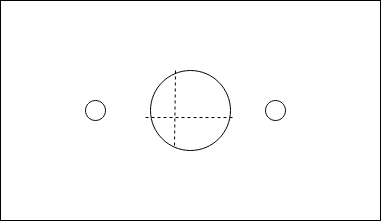
\includegraphics[scale=0.5]{img/verschobenes_werkstueck}\\
\end{center}

Die schraffierten Linien sollten den Sollwert des Zentrums darstellen. In diesem Fall wäre es möglich
in einer sogenannten Spiralsuche nach der Fügeposition zu suchen um das Fügeteil schlussendlich einzusetzen.
\newpage
\item 
Wenn das Werkstück nicht vollständig eben aufliegt

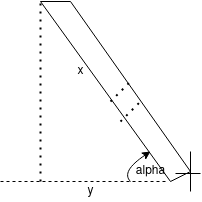
\includegraphics[scale=0.8]{img/winkel_werkstueck}\\

Hier sollte die Summe der Kräfte und Drehmomente nicht null sein, da, dass Fügeelement nicht eben auf dem Werkstück liegt. Somit sollte sich der Manipulator so bewegen bis die oben besagten physikalischen Eigenschaften in Summe null ergeben, anschließend kann mit der Spiralsuche fortgeführt werden. Es gilt hier weiter zu untersuchen welches Regelungskonzept wie es in Kapitel 2.1 erwähnt wurden sich für die Bewältigung der Füge Aufgabe besser eignet.
\end{itemize}


\section{Literaturliste}
\begin{itemize}
\item[] [1] Alexander Winkler: Sensorgeführte Bewegung stationärer Roboter. Universitätsverlag Chemnitz, 2016, S. 37
\item[] [2] https://de.wikipedia.org/wiki/Kraftregelung: Aktive Impedanzregelung
\item[] [3] Alexander Winkler: Sensorgeführte Bewegung stationärer Roboter. Universitätsverlag Chemnitz, 2016, S. 40
\end{itemize}

\end{document}